\documentclass[conference]{IEEEtran}
\IEEEoverridecommandlockouts
% The preceding line is only needed to identify funding in the first footnote. If that is unneeded, please comment it out.
\usepackage{cite}
\usepackage{amsmath,amssymb,amsfonts}
\usepackage{algorithmic}
\usepackage{graphicx}
\usepackage{textcomp}
\usepackage{xcolor}
\usepackage{gensymb}
\usepackage{listings}
\usepackage[framed,numbered,autolinebreaks,useliterate]{mcode}
\def\BibTeX{{\rm B\kern-.05em{\sc i\kern-.025em b}\kern-.08em
    T\kern-.1667em\lower.7ex\hbox{E}\kern-.125emX}}
\begin{document}

\title{RBE 501 Week 2 Assignment}

\author{\IEEEauthorblockN{1\textsuperscript{st} Arjan Gupta}
\IEEEauthorblockA{\textit{Robotics Engineering} \\
\textit{Worcester Polytechnic Institute}\\
Worcester, MA, USA \\
agupta11@wpi.edu}
}

\maketitle

\begin{abstract}
This document provides an in-depth solution for Problems 3--2 and 3--5 described 
in the Robot Modeling and Control textbook.
This is the assignment for the second week in RBE 501 (Robot Dynamics),
Spring 2023 at Worcester Polytechnic Institute.
\end{abstract}

\begin{IEEEkeywords}
robotics, forward kinematics, manipulator
\end{IEEEkeywords}

\section{Introduction}
We are asked to solve Problems 3--2 and 3--5 of the main textbook~\cite{Spong2006}.
For Problem 3--2, the objective is to calculate the forward kinematic equations
of the robot shown in Figure 1 below, \textit{without} using the DH-convention.\\
\begin{figure}[h]
    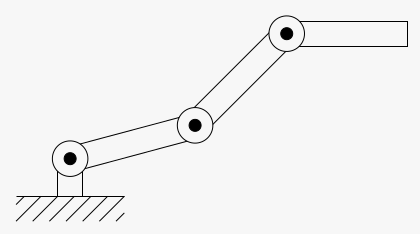
\includegraphics[scale=0.4]{prob3_2.png}
    \centering
    \caption{Three-link planar arm of Problem 3--2}
\end{figure}\\
For Problem 3--5, the objective is to calculate the forward kinematic equations
of the robot shown in Figure 2 below, using the DH-convention.
\begin{figure}[h]
    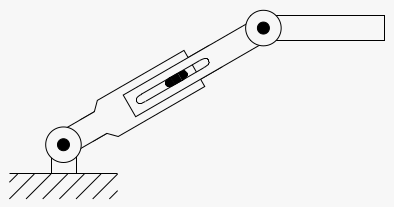
\includegraphics[scale=0.4]{prob3_5.png}
    \centering
    \caption{Three-link planar arm with prismatic joint of Problem 3--5}
\end{figure}

\section{Materials and Methods}

\subsection{Approach for Problem 3--2}

\subsubsection{Restate objective in technical terms}
In technical terms, we must first assign frames 0 through 3 for
each link of the manipulator. Then, we need to find the homogeneous
transformation matrices between each frame, i.e.\ we need to find
$H^0_1$, $H^1_2$, and $H^2_3$. Using these, we need to find $H^0_3$
to give us our final answer.

\subsubsection{Assign frames}
The first step toward solving our problem is to redraw our robot in symbolic
form, and assign frames for links 0 through 3. This is shown in
Figure 3. Frame 0 ($x_0 y_0 z_0$) is assigned at the first joint, frame 1
($x_1 y_1 z_1$) is assigned at the
second joint, and frame 2 ($x_2 y_2 z_2$)
 is assigned at third joint. All joints in this case are revolute.
 Frame 3 ($x_3 y_3 z_3$) is assigned at
the end of link 3.\\
% \vspace{0in}\\
\begin{figure}[h]
    \centering
    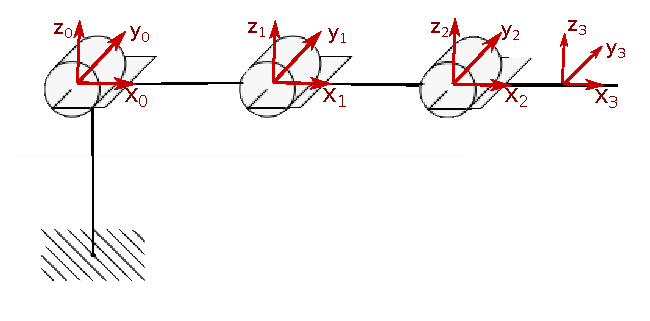
\includegraphics[scale=0.8]{prob3_2_redraw}
    \caption{Symbolic form of Figure 1, along with frame assignments}
    \setlength{\belowcaptionskip}{-50pt}
\end{figure}
\subsubsection{Variables and constants}
Now that we have assigned the frames, we can come up with some constants for
the link lengths. Assume that link 1 is of constant length $L_1$, link 2 is 
of constant length $L_2$, and link 3 is of constant length $L_3$. Additionally,
we are dealing with 3 revolute joints, so when the first revolute joint moves,
an angle subtended by $x_1$ from $x_0$ is the variable $\theta_1$. Similarly,
when the second and third revolute joints move, we get a variable angles of
$\theta_2$ and $\theta_3$.

\subsubsection{Find H matrices}
We can now start formulating our homogeneous transformation matrices.

We first form the rotation matrices. The rotation matrices are given by
the angle of rotation $\theta$ about the Y axis, given as the following.
\begin{equation*}
    R_y =
    \begin{bmatrix}
         \cos\theta  & 0 & \sin\theta\\
         0 & 1 & 0\\
         -\sin\theta & 0 & \cos\theta
    \end{bmatrix}
\end{equation*}

In our Live Script, we use the following MATLAB code to formulate $R_y$.

\lstinputlisting{formulate_ry.m}

Since all our link lengths are constants along the x-axis of the
respective frames, they take on the following form.

\begin{equation*}
    d = \begin{bmatrix}
        L \cos\theta\\0\\L\sin\theta
    \end{bmatrix}
\end{equation*}

This can again be turned into a function, as follows.

\lstinputlisting{formulate_d_prob3_2.m}

Furthermore, we use another handy function to compute the homogeneous
transformation matrices.

\lstinputlisting{compute_h.m}

Using this function and the previous ones,
we found the following H matrices for the frame-to-frame transformations.

\[
    H^0_1 = \begin{bmatrix}
        R^0_1 & d^0_1\\
        0 & 1
    \end{bmatrix}
    =
    \begin{bmatrix}
        \cos\theta _{1} & 0 & \sin\theta _{1} & L_{1} \cos\theta_1\\
        0 & 1 & 0 & 0\\
        -\sin\theta _{1} & 0 & \cos\theta_{1} & L_1 \sin\theta_1\\
        0 & 0 & 0 & 1
    \end{bmatrix}
\]

\[
    H^1_2 = \begin{bmatrix}
        R^1_2 & d^1_2\\
        0 & 1
    \end{bmatrix}
    =
    \begin{bmatrix}
        \cos\theta _{2} & 0 & \sin\theta _{2} & L_{2} \cos\theta_2\\
        0 & 1 & 0 & 0\\
        -\sin\theta _{2} & 0 & \cos\theta_{2} & L_2 \sin\theta_2\\
        0 & 0 & 0 & 1
    \end{bmatrix}
\]

\[
    H^2_3 = \begin{bmatrix}
        R^2_3 & d^2_3\\
        0 & 1
    \end{bmatrix}
    =
    \begin{bmatrix}
        \cos\theta _{3} & 0 & \sin\theta _{3} & L_{3} \cos\theta_3\\
        0 & 1 & 0 & 0\\
        -\sin\theta _{3} & 0 & \cos\theta_{3} & L_3 \sin\theta_3\\
        0 & 0 & 0 & 1
    \end{bmatrix}
\]

Now we are ready to multiply these matrices to obtain the final result
of our objective.

\subsection{Approach for Problem 3--5}

\subsubsection{Restate objective in technical terms}
In technical terms, we must first assign frames 0 through 3 for
each link of the manipulator. We will then form a table of DH
parameters. Using the table, and the general form of the DH matrix,
we will find the $A$ matrices for the manipulator i.e.\ we need to find
$A_1$, $A_2$, and $A_3$. Using these, we need to find $T^0_3$
to give us our final answer. From our textbook~\cite{Spong2006}, the 
DH Coordinate Frame Assumptions are,
\begin{itemize}
    \item \textbf{(DH1)} The axis $x_1$ is perpendicular to the axis $z_0$.
    \item \textbf{(DH2)} The axis $x_1$ intersects the axis $z_0$.
\end{itemize}
\vspace{0.1in}
\begin{figure}[h]
    \centering
    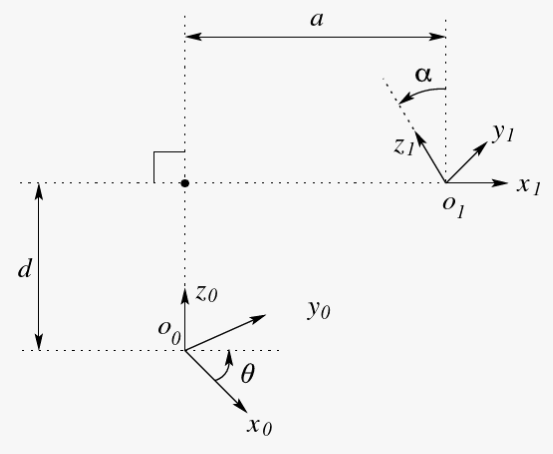
\includegraphics[scale=0.4]{dh-frames.png}
    \caption{Coordinate frames satisfying DH assumptions}
\end{figure}
\vspace{0.1in}
\subsubsection{Assign frames}
The first step toward solving our problem is to redraw the robot
manipulator in symbolic
form, and assign frames for links 0 through 3. Since we are following the DH assumptions,
we must follow the frame assignment style shown in Figure 4, which
is from our textbook~\cite{Spong2006}. Our redrawn figure is shown in Figure 5.\\
\begin{figure}[h]
    \centering
    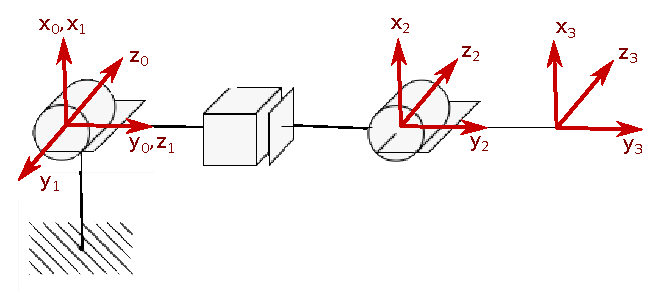
\includegraphics[width=3.4in]{prob3_5_redraw}
    \caption{Figure 2 redrawn in symbolic form with frames assigned}
\end{figure}\\
As shown, frame 0 ($x_0 y_0 z_0$) is assigned at the first joint (revolute). Frame 1
($x_1 y_1 z_1$) is also assigned at the
first joint in order to have DH assumptions satisfied. Frame 2 ($x_2 y_2 z_2$)
 is assigned at third joint (revolute). Frame 3 ($x_3 y_3 z_3$) is assigned at
the end of link 3.\\

\subsubsection{Create DH table and set variables/constants}
Now that we have assigned the frames, we can use Figure 4 to write
the $\alpha_i$, $a_i$, $\theta_i$, $d_i$ quantities for each link.

\begin{table}[h!]
    \begin{center}
        \resizebox{0.7\columnwidth}{!}{%
        \begin{tabular}{||c|c|c|c|c||}
        \hline
        Link & $\alpha_i$ & $a_i$ & $\theta_i$ & $d_i$ \\
        \hline\hline
        1 & $-90\degree$ & 0 & $\theta_1$ & 0 \\
        2 & $90\degree$ & 0 & 0 & $L_1 + q_2$ \\
        3 & 0 & $L_3$ & $\theta_3$ & 0\\
        \hline
        \end{tabular}
        }
    \end{center}
    \caption{Denavit-Hartenberg table for Problem 3--5}
\end{table}

As seen in Table 1, we have chosen $L_1$ and $L_3$ to describe the constant link
lengths of links 1 and 3, respectively. Additionally, $q_2$ describes the variable
link length of link 2 (because of joint 2 being a prismatic joint).
Furthermore, $\theta_1$ and $\theta_3$ describe the
variable angles of revolute joints 1 and 3, respectively.

\subsubsection{Find $A$ matrices}

As given in our textbook~\cite{Spong2006}, the general form of an
$A_i$ matrix is,

\[
    A_i =
    \begin{bmatrix}
        c_{\theta_i} & -s_{\theta_i}c_{\alpha_i} & s_{\theta_i}s_{\alpha_i} & a_i c_{\theta_i}\\
        s_{\theta_i} & c_{\theta_i}c_{\alpha_i} & -c_{\theta_i}s_{\alpha_i} & a_i s_{\theta_i}\\
        0 & s_{\alpha_i} & c_{\alpha_i} & d_i\\
        0 & 0 & 0 & 1
    \end{bmatrix}
\]

Where $c_{\theta_i}$ is $\cos{\theta_i}$, $s_{\theta_i}$ is $\sin{\theta_i}$,
$c_{\alpha_i}$ is $\cos{\alpha_i}$, and $s_{\alpha_i}$ is $\sin{\alpha_i}$.
We can write a MATLAB function for this $A_i$ matrix, as follows.

\lstinputlisting{compute_dh_a.m}

Using this function in our MATLAB Live Script, we produce the following A matrices.

\[
    A_1 =
    \begin{bmatrix}
        \cos \theta_1 & 0 & -\sin \theta_1 & 0\\
        \sin \theta_1 & 0 & \cos  \theta_1 & 0\\
        0 & -1 & 0 & 0\\
        0 & 0 & 0 & 1
        \end{bmatrix}
\]

\[
    A_2 = 
    \begin{bmatrix}
        1 & 0 & 0 & 0\\
        0 & 0 & -1 & 0\\
        0 & 1 & 0 & L_1 + q_2 \\
        0 & 0 & 0 & 1
        \end{bmatrix}
\]

\[
    A_3 =
    \begin{bmatrix}
        \cos \theta_3 & -\sin \theta_3 & 0 & L_3 \,\cos \theta_3\\
        \sin \theta_3 & \cos  \theta_3 & 0 & L_3 \,\sin \theta_3\\
        0 & 0 & 1 & 0\\
        0 & 0 & 0 & 1
        \end{bmatrix}
\]

Now we are ready to multiply these matrices to obtain the final result
of our objective.

\section{Results}

\subsection{Result for Problem 3--2}

For Problem 3--2, we obtained our final result by multiplying all three $H$ matrices
that we obtained in the Materials and Methods section. Hence, we obtained the following
matrix,
\[
    H^0_3 =
    \begin{bmatrix}
    \sigma_1  & 0 & \sigma_5  & \lambda_1 \\
    0 & 1 & 0 & 0\\
    \sigma_4 & 0 & \sigma_1  & \lambda_2 \\
    0 & 0 & 0 & 1
    \end{bmatrix}
\]

where,
\begin{multline*}
    \lambda_1 = L_1 \,\cos \left(\theta_1 \right)+L_3 \,\cos \left(\theta_3 \right)\,\sigma_2 \\+L_3 \,\sin \left(\theta_3 \right)\,\sigma_3 +L_2 \,\cos \left(\theta_1 \right)\,\cos \left(\theta_2 \right)\\+L_2 \,\sin \left(\theta_1 \right)\,\sin \left(\theta_2 \right)\\
    \\
    \lambda_2 = L_1 \,\sin \left(\theta_1 \right)-L_3 \,\cos \left(\theta_3 \right)\,\sigma_3 +L_3 \,\sin \left(\theta_3 \right)\,\sigma_2 \\+L_2 \,\cos \left(\theta_1 \right)\,\sin \left(\theta_2 \right)-L_2 \,\cos \left(\theta_2 \right)\,\sin \left(\theta_1 \right)
\end{multline*}
\hspace{10pt} and,
\begin{align*}
    \sigma_1 &=\cos \left(\theta_3 \right)\,\sigma_2 -\sin \left(\theta_3 \right)\,\sigma_3 \\
    \sigma_2 &=\cos \left(\theta_1 \right)\,\cos \left(\theta_2 \right)-\sin \left(\theta_1 \right)\,\sin \left(\theta_2 \right)\\
    \sigma_3 &=\cos \left(\theta_1 \right)\,\sin \left(\theta_2 \right)+\cos \left(\theta_2 \right)\,\sin \left(\theta_1 \right)\\
    \sigma_4 &= -\cos \left(\theta_3 \right)\,\sigma_3 -\sin \left(\theta_3 \right)\,\sigma_2\\
    \sigma_5 &= \cos \left(\theta_3 \right)\,\sigma_3 +\sin \left(\theta_3 \right)\,\sigma_2
\end{align*}

This result is best visualized within the MATLAB Live Script that has been submitted 
alongside this report.

\subsection{Result for Problem 3--5}

For Problem 3--5, we obtained our final result by multiplying all three $A_i$ matrices
that we obtained in the Materials and Methods section. Hence, we obtained the following
matrix,

$\begin{array}{l}
    \left(\begin{array}{cccc}
    \sigma_1  & -\sigma_3 -\sigma_2  & 0 & L_3 \,\cos \left(\theta_1 \right)\,\cos \left(\theta_3 \right)-\sin \left(\theta_1 \right)\,{\left(L_1 +q_2 \right)}-L_3 \,\sin \left(\theta_1 \right)\,\sin \left(\theta_3 \right)\\
    \sigma_3 +\sigma_2  & \sigma_1  & 0 & \cos \left(\theta_1 \right)\,{\left(L_1 +q_2 \right)}+L_3 \,\cos \left(\theta_1 \right)\,\sin \left(\theta_3 \right)+L_3 \,\cos \left(\theta_3 \right)\,\sin \left(\theta_1 \right)\\
    0 & 0 & 1 & 0\\
    0 & 0 & 0 & 1
    \end{array}\right)\\
    \mathrm{}\\
    \textrm{where}\\
    \mathrm{}\\
    \;\;\sigma_1 =\cos \left(\theta_1 \right)\,\cos \left(\theta_3 \right)-\sin \left(\theta_1 \right)\,\sin \left(\theta_3 \right)\\
    \mathrm{}\\
    \;\;\sigma_2 =\cos \left(\theta_3 \right)\,\sin \left(\theta_1 \right)\\
    \mathrm{}\\
    \;\;\sigma_3 =\cos \left(\theta_1 \right)\,\sin \left(\theta_3 \right)
    \end{array}$

\section{Discussion}
In the opinion of the author, this homework problem set was insightful. The
first problem proved that we do not need to always use the DH convention
when solving for forward kinematics in robotic manipulators. In fact, when
using tools like MATLAB, to using a non-DH method of
computing the forward kinematics is no more complex than using the DH method
itself.\\\\
The second problem reinforced our learnings from RBE 500. We used the DH
convention heavily in that class, so it was great to revisit that foundation
as we move forward in this class.\\\\
A topic for further consideration could be, when would one prefer to use
a non-DH method over the DH method? The DH convention can provide a minimal
and efficient way to represent and compute the relationship between the base
frame and the end effector in many cases, because it reduces the number of
variables involved from 6 to 4. However, suppose we want to model the
differential kinematics of a manipulator. The screw-based theory~\cite{Rocha2011}
can provide advantages in such a case. It was found that, when
various kinematic modelings for common manipulator configurations where
compared, the screw-based theory did not provide any disadvantages in any
case. The one noticeable difference was that it provided superior flexibility
when differential kinematics was compared.
The parameter identification is also a bit simpler in the screw-based theory, as
compared to the DH-convention.
\bibliography{refs.bib}
\bibliographystyle{IEEEtran}

\end{document}